 \section{Experiment Apparatus:  The ATLAS Detector at the LHC}

\subsection{The Large Hadron Collider} 
The Large Hadron Collider (LHC) \cite{LHC} is a 27 km long circular proton accelerator embedded underground of the Geneva area.
%and Frech villages overviewing the Mont Blanc \cite{MontBlanc}.
It is designed to collide protons at a center-of-mass energy of $\sqrt{s} = 14 \tev$, at the four detector cites (ATLAS\cite{ATLAS_exp}, CMS\cite{CMS}, ALICE\cite{ALICE} and LHCb\cite{LHCb}) built on the accelerator ring. ATLAS and CMS are general purpose detectors designed to study a vast range of physics programs, while LHCb and ALICE are specialized in studying b-hadrons and heavy-ion collisions respectively. \\

The operation started in 2010, offering proton-proton (pp) collisions at a center-of-mass energies of $7\tev$ and $8\tev$ with $4.7\ifb$ and $20.3\ifb$ of integrated luminosity until 2012 (Run1). The center-of-mass energies has been almost doubled to $13\tev$
in the runs starting from 2015 (Run2). The LHC has also delivered lead-ion (Pb-Pb) collisions with a center-of-mass energy of $\sqrt{s_{NN}} = 2.76\tev$ and proton-lead (p-Pb) collisions with $\sqrt{s_{NN}} = 5.02\tev$.

% In a chamber, 
% 

% The protons are then accelerated (段階的に) sequently through the booster accelerator (linac, PS, SPS) and finally injected into LHC. 
% In LHC

% number of pileup
The acceleration of protons stages into various steps: 
Protons are firstly seeded from hydrogen gas, by blowing off the electrons from the hydrogen atoms using high electric field.
They are injected in the linear accelerator LINAC2 with accelerated upto 50 MeV, and sent into the Proton Synchrotron Booster (PSB) being accelerated up to an energy of 1.4 GeV. 
The subsequent accelerator is the Proton Synchrotron (PS) elevating the energy of the protons to $25\gev$, and injecting them into the Super Proton Synchrotron (SPS). After being accelerated to $450\gev$ in SPS, the protons finally enter the two LHC beam pipes running the beam oppositely each other. The acceleration chain is illustrated in Fig. \ref{fig::Detector::LHC}.

\fig[170]{Detector/LHC_schematic.pdf}
{LHC. \cite{LHCPhoto}}
{fig::Detector::LHC}


The LHC accelrator consists of octant-shaped 2.45 km arcs with 1232 superconducting magnets located at the curves, providing 8.33T of magnetic field to bend the proton trajectory.
%They are operated at 1.9K cooled by liquid-helium, 
In total, 39 crossing-trains can be filled into the LHC simultaneously in a design conditions, with 2808 crossinges per beam are brought to collision in the LHC. Each crossing contains about $10^{11}$ protons. 
The beam crossinges are collided with a beam crossing angle of 285 mrad. 
The peak luminosity amounts upto $L = 0.7-1.4 \times 10^{34} \mathrm{cm}^{2} \mathrm{s}^{-1}$ in the 2015-2016 runs, as shown in Fig. \ref{fig::Detector::DAQ} (a).

Due to the high frequency of collisions and the dense proton crossinges, multiple proton collisions can take place simultaneously within the same crossing crossing, referred as ``pile-up''. 
% to maximizing the chance of interesting reaction 
The average pile-up $\mu$, defined as the mean number of interactions per crossing crossing,  
has been evolved according to the peak luminosity increase, amounting to $20-40$ in recent runs in 2016. The $\mu$ profile is shown in Fig. \ref{fig::Detector::DAQ} (b).

%%%%%%%%%
\begin{figure}[h]
  \centering
    \subfigure[]{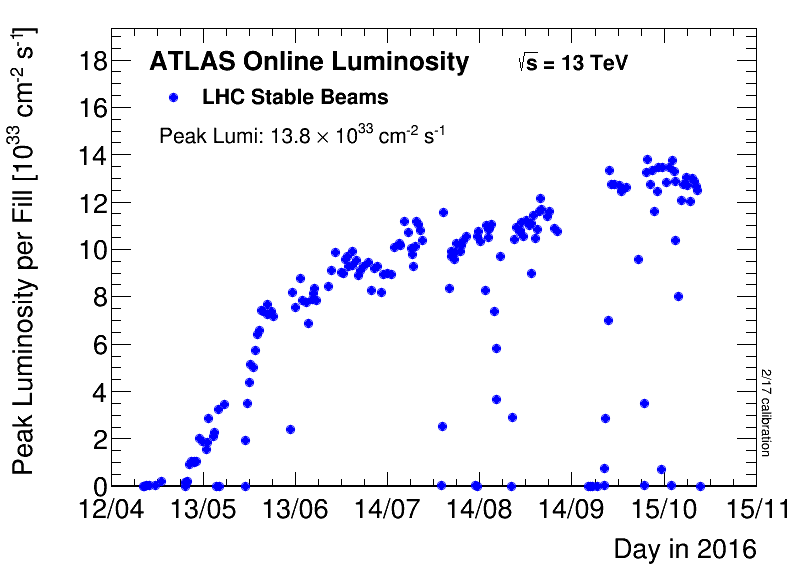
\includegraphics[width=0.48\textwidth]{figures/Detector/peakLumi2016.png}}
    \subfigure[]{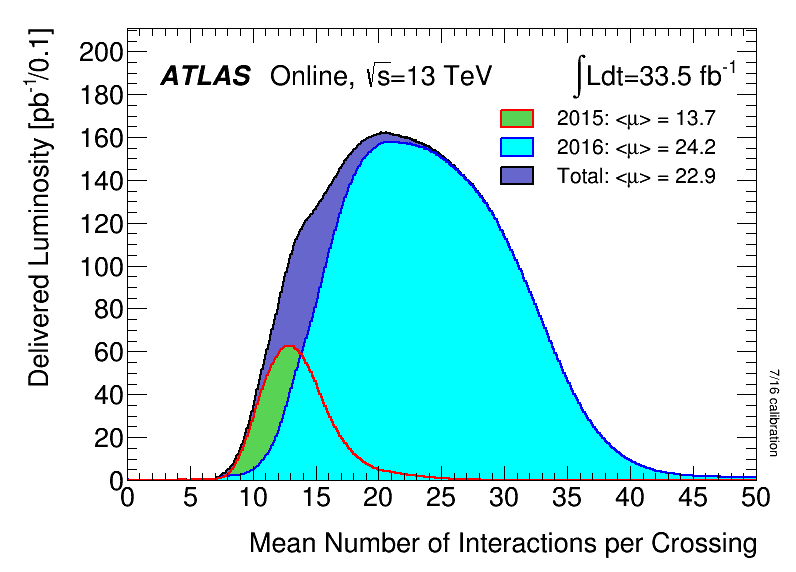
\includegraphics[width=0.48\textwidth]{figures/Detector/mu_2015_2016.png}}
    \caption{  (a) Peak luminosity evolution in 2016 runs \cite{DAQ2016}, and (b) the pile-up profile obtained in 2015-2016 runs  \cite{lumiPubResult}.
      \label{fig::Detector::DAQ}
    }
\end{figure}
%%%%%%%%%%



%and are categorized as in-time or out-of-time pile-up. In-time pile-up events are caused by additional interactions of protons in the same crossing collision. The out-of-time pile-up occurs when traces from an event in a different crossing-crossing are recorded. 


%%%%%%%%%%%%%%%%%%%%%%%%%%%%%%%%%%%%%%%%%%%%%%%%%%%%%%%%%
\subsection{Particle Measurement and The ATLAS Detector}
ATLAS (A Toroidal LHC ApparatuS) is a general purpose detector, aiming to probe a wide range of physics programs from precision measurements of EW physics to the energy frontier experiments, through a dedicated measurement of particles produced in $pp$ collisions. The detector spans over 44m in width and stand 25m in height, covering the interaction point (IP) by a cylindrical barrel and two endcaps, achieving a nearly full solid angle coverage. The total weight amounts 7000 tons including stopping materials to fully accommodate the produced particles, enabling complete measurement of particle energy. The cut-away image is shown in Fig. \ref{fig::Detector::ATLAS_whole}. \\

The purposes of the detector are mainly two-fold:
\begin{itemize}
\item identification of particle species,
\item determination of particle's energy and momentum,
\end{itemize}
with two complemental concepts of measurement:
\begin{itemize}
\item fast measurement for providing trigger
\item precision measurement of particle properties
\end{itemize}
 
To satisfy these functionalities at the same time, following sub-detectors are arranged in a designed order from the innermost toward outside with respect to the IP.

\begin{itemize}
\item Inner detector (and magnets) to identify and measure electrically charged particles, as well as define the primary vertices. \\
Charged particle can easily interact with materials by ionizing the molecules inside. The path of flight can be ``imaged'' as a track, by recording the position of ionization. 
In ATLAS, a complex of discrete layers of silicon sensors and a continuously volumed gas chambers are placed in the innermost. 
The momentum can be measured in addition by applying magnetic field, and quantifying the curvature of the bent trajectory. 

\item Calorimeters to measure the energy of electron, photon and hadrons. \\
Electrons and photons traveling inside materials above certain energy 
\footnote{Referred to the critical energy. $\sim 800 \mev$ for typical material.}
lose their energy through electromagnetic showering; photons create $e^+e^-$ pairs and electrons spew bremsstrahlung photon; 
the daughter electrons and photons are multiplicated by this recursive repetition; ending up in a particle shower. 
Most of the energy are absorbed after traversing about 20 radiation lengths ($X_0$) of material. 
Hadrons (mostly pions) also cause similar cascade reactions. 
The shower branch evolves by interacting with nucleus in the material via strong interaction, meanwhile produced $\pi_0$s promptly decay into two photons which shower electromagneticly. 
The resultant shower is combination of a long hadronic shower and small local EM clusters in it. 
Electromagnetic and hadronic calorimeters are set as the outer layers of the trackers, to measure such showers by absorbing them in it.\\

\item Muon spectrometer (and the magnet) to measure the muons penetrating the detector. \\
Among all the particles that interact with material, muons are only exception who do not seriously deposit the energy in calorimeter. 
This is due to the fact that muons happen to have the mass realizing the minimum EM interaction with material (Minimum Ionizing Particle; MIP), 
and the corresponding critical energy for EM showering is usually at several TeV level.
%, surpassing the typical energy range of particles generated in LHC. 
This is actually a lovely coincident for human being (or poor particle physicists), 
since they can be easily identified i.e. particles punching through the calorimeter are automatically muons. The muon spectrometer located outermost serves for identifying such muons as well as measuring the tracks together with the inner tracker described above.

\item Given the total momentum conservation in transverse direction in each collision, 
the presence of non-interacting particles such as neutrinos and hypothetical new particles can be indirectly detected through the imbalance; 
This is referred to missing $\ET$ ($\met$), 
\footnote{The ``$\ET$'' in the name is due to a historical reason; it used to be calculated only using calorimeter deposits, which is now actually outdated. 
Also, momentum and energy effectively give no differences for most of detected particles in LHC, since their energy typically overwhelms the masses.}
defined by the negative of the vectoral sum of transverse momentum of all detected particles.
\end{itemize}


In the following subsections, each of the sub-detector system will be overviewed, comprehensively based on references \cite{ATLAS_exp} and \cite{ATLAS_TDR}.

\fig[110]{Detector/figures_AtlasDetectorLabelled.png}
{Full-body view of the ATLAS detector \cite{ATLAScosmicPerf}. The geometry is completely forward-back symmeric.}
{fig::Detector::ATLAS_whole}


%%%%%%%%%%%%%%%%%%%%%%%%%%%%%%%%%%%%%%%%%%%%%%%%%%%%%%%%%
\subsubsection{Coordinate System}
For referencing the position of the detector as well as the orientation of particles, a right-handed Cartesian coordinate system is defined with the interaction point being the origin and the x-axis pointing to the center of the LHC ring. The y,z-axes are accordingly the direction of sky or the beam direction respectively. Polar angle $\theta$ and azimuthal angle $\phi$ are defined by the cylindrical representation $(\theta,\phi,z)$: $\theta$ ranges from 0 to $2\pi$ with respect to the z-axis, and $\phi$ runs from $-\pi$ to $\pi$ from the x-axis. The two endcaps in the ATLAS detector are referred as ``A-side'' and ``C-side'', corresponding to the position of positive and negative coordinate in the z-axis. \\

It is the unfortunate fate for hadron colliders that particles generated by collisions are usually highly boosted along z-axis, since the energy of the initial interacting partons inside the hardons are asymmetric. From this point of view, a set of variables with Lorentz-invariant nature are introduced for describing momentum or position. In particular, it is useful to define the transverse component of variables, such as transverse momentum $\pt := p\sin{\theta}$ or transverse energy $E := E\sin{\theta}$. The advantage over the use of $p$ or $E$ is obvious that they do express the intrinsic hardness of the particles in the center-of-mass frame of the reaction, and also that the vectoral sum of all particles conserves before and after the collision. \\

Similarly, pseudo-rapidity $\eta$ defined below commonly serves as the coordinate of polar angle:
\begin{align}
\eta := \ln \left( \log{\frac{\theta}{2}} \right).
\end{align}
It has two practical advantages over $\theta$ the difference in pseudo-rapidity between particles $\Delta\eta$ are invariant against the boost towards z-direction. 
\footnote{
This is true when the particles are massless, which is approximately valid given that the boos along z-axis is sourced by the momentum of order of the beam energy.}
; $\eta$ has an effectively finer measure at very forward direction where $\theta$ suffers from the degeneracy i.e. $\cos{\theta}\sim 1$, thus more convenient in expressing the orientation of forward particles.

Angular distance between two particles are commonly expressed by $R$ that is defined as: 
\begin{align}
\Delta R := \sqrt{(\Delta\eta)^2+(\Delta\phi)^2}.
\end{align}

%\fig[110]{Detector/ACside.pdf}{.}{fig::Detector::ACside}


%%%%%%%%%%%%%%%%%%%%%%%%%%%%%%%%%%%%%%%%%%%%%%%%%%%%%%%%%
\subsubsection{Inner Detectors}
The inner detector (ID) is placed the inner-most of the ATLAS detector, designed to measure the tracks of charged particles, 
as well as precisely determining the position of vertices of the hardest scattering in interest.

It consists of a silicon tracker (the pixel detector and the semiconductor tracker ;SCT) at the inner radii,
and the Transition Radiation Tracker (TRT) for continuous tracking at the outer radii. 
The detector arrangement is illustrated in Fig. \ref{fig::Detector::innerDetector_xsec} and Fig. \ref{fig::Detector::innerDetector}.
The outer radius is surrounded by the central solenoid, providing a magnetic field of 2T along the $z$-axis,
to bend the tracks traveling inside the ID volume.
%The general requirement for tracking is the fine granularity of detector segmentation, to achieve high resolution of track momentum as well as quality measurement. 
% as a result, number of channel skyrocket.
%high position resolution 
% trackのresolutionは内側の方が1点あたりのresolution impactが大きいので, 内側ほどgranularityの高いsub-detectorを置いている

% \footnote{Ideally pixelで全部被覆できれば最高であるが、costがr^2でscaleしてとんでもないことになるのでcostとbest compromizeした結果今のようになった。それでもchannel数, 被覆面積は...であり、crazyの極致である。}

% 基本的にチャネルが多くて読み出しに時間がかかるのでR&D purposeを除いてtriggerは発行していない
%
%%%
% 後段のcaloのmeasurementを邪魔しないために、materialはminimizeされてる
As a general requirement, ID has to contain material as less as possible, to avoid disturbing the measurement downstream by the energy loss. 
Fig. \ref{fig::Detector::IDmaterial} shows the total material profile of the ID over $|\eta|$. 
The material volume is suppressed below $2.5$ radiation length and 1 nucleus interaction length, which is low enough compared with energy dropped in the calorimeter.


%%%%%%%%%
\fig[110]{Detector/innerDetector_xsec.pdf}
{Cross-section of the ATLAS inner detectors \cite{ATLAS_exp}.}
{fig::Detector::innerDetector_xsec}


\fig[110]{Detector/ATLAS_innerDetector.jpg}
{Cut-away view of the ATLAS inner-detector \cite{ATLAS_exp}.}
{fig::Detector::innerDetector}

%%%%%%%%%
\begin{figure}[h]
  \centering
    \subfigure[]{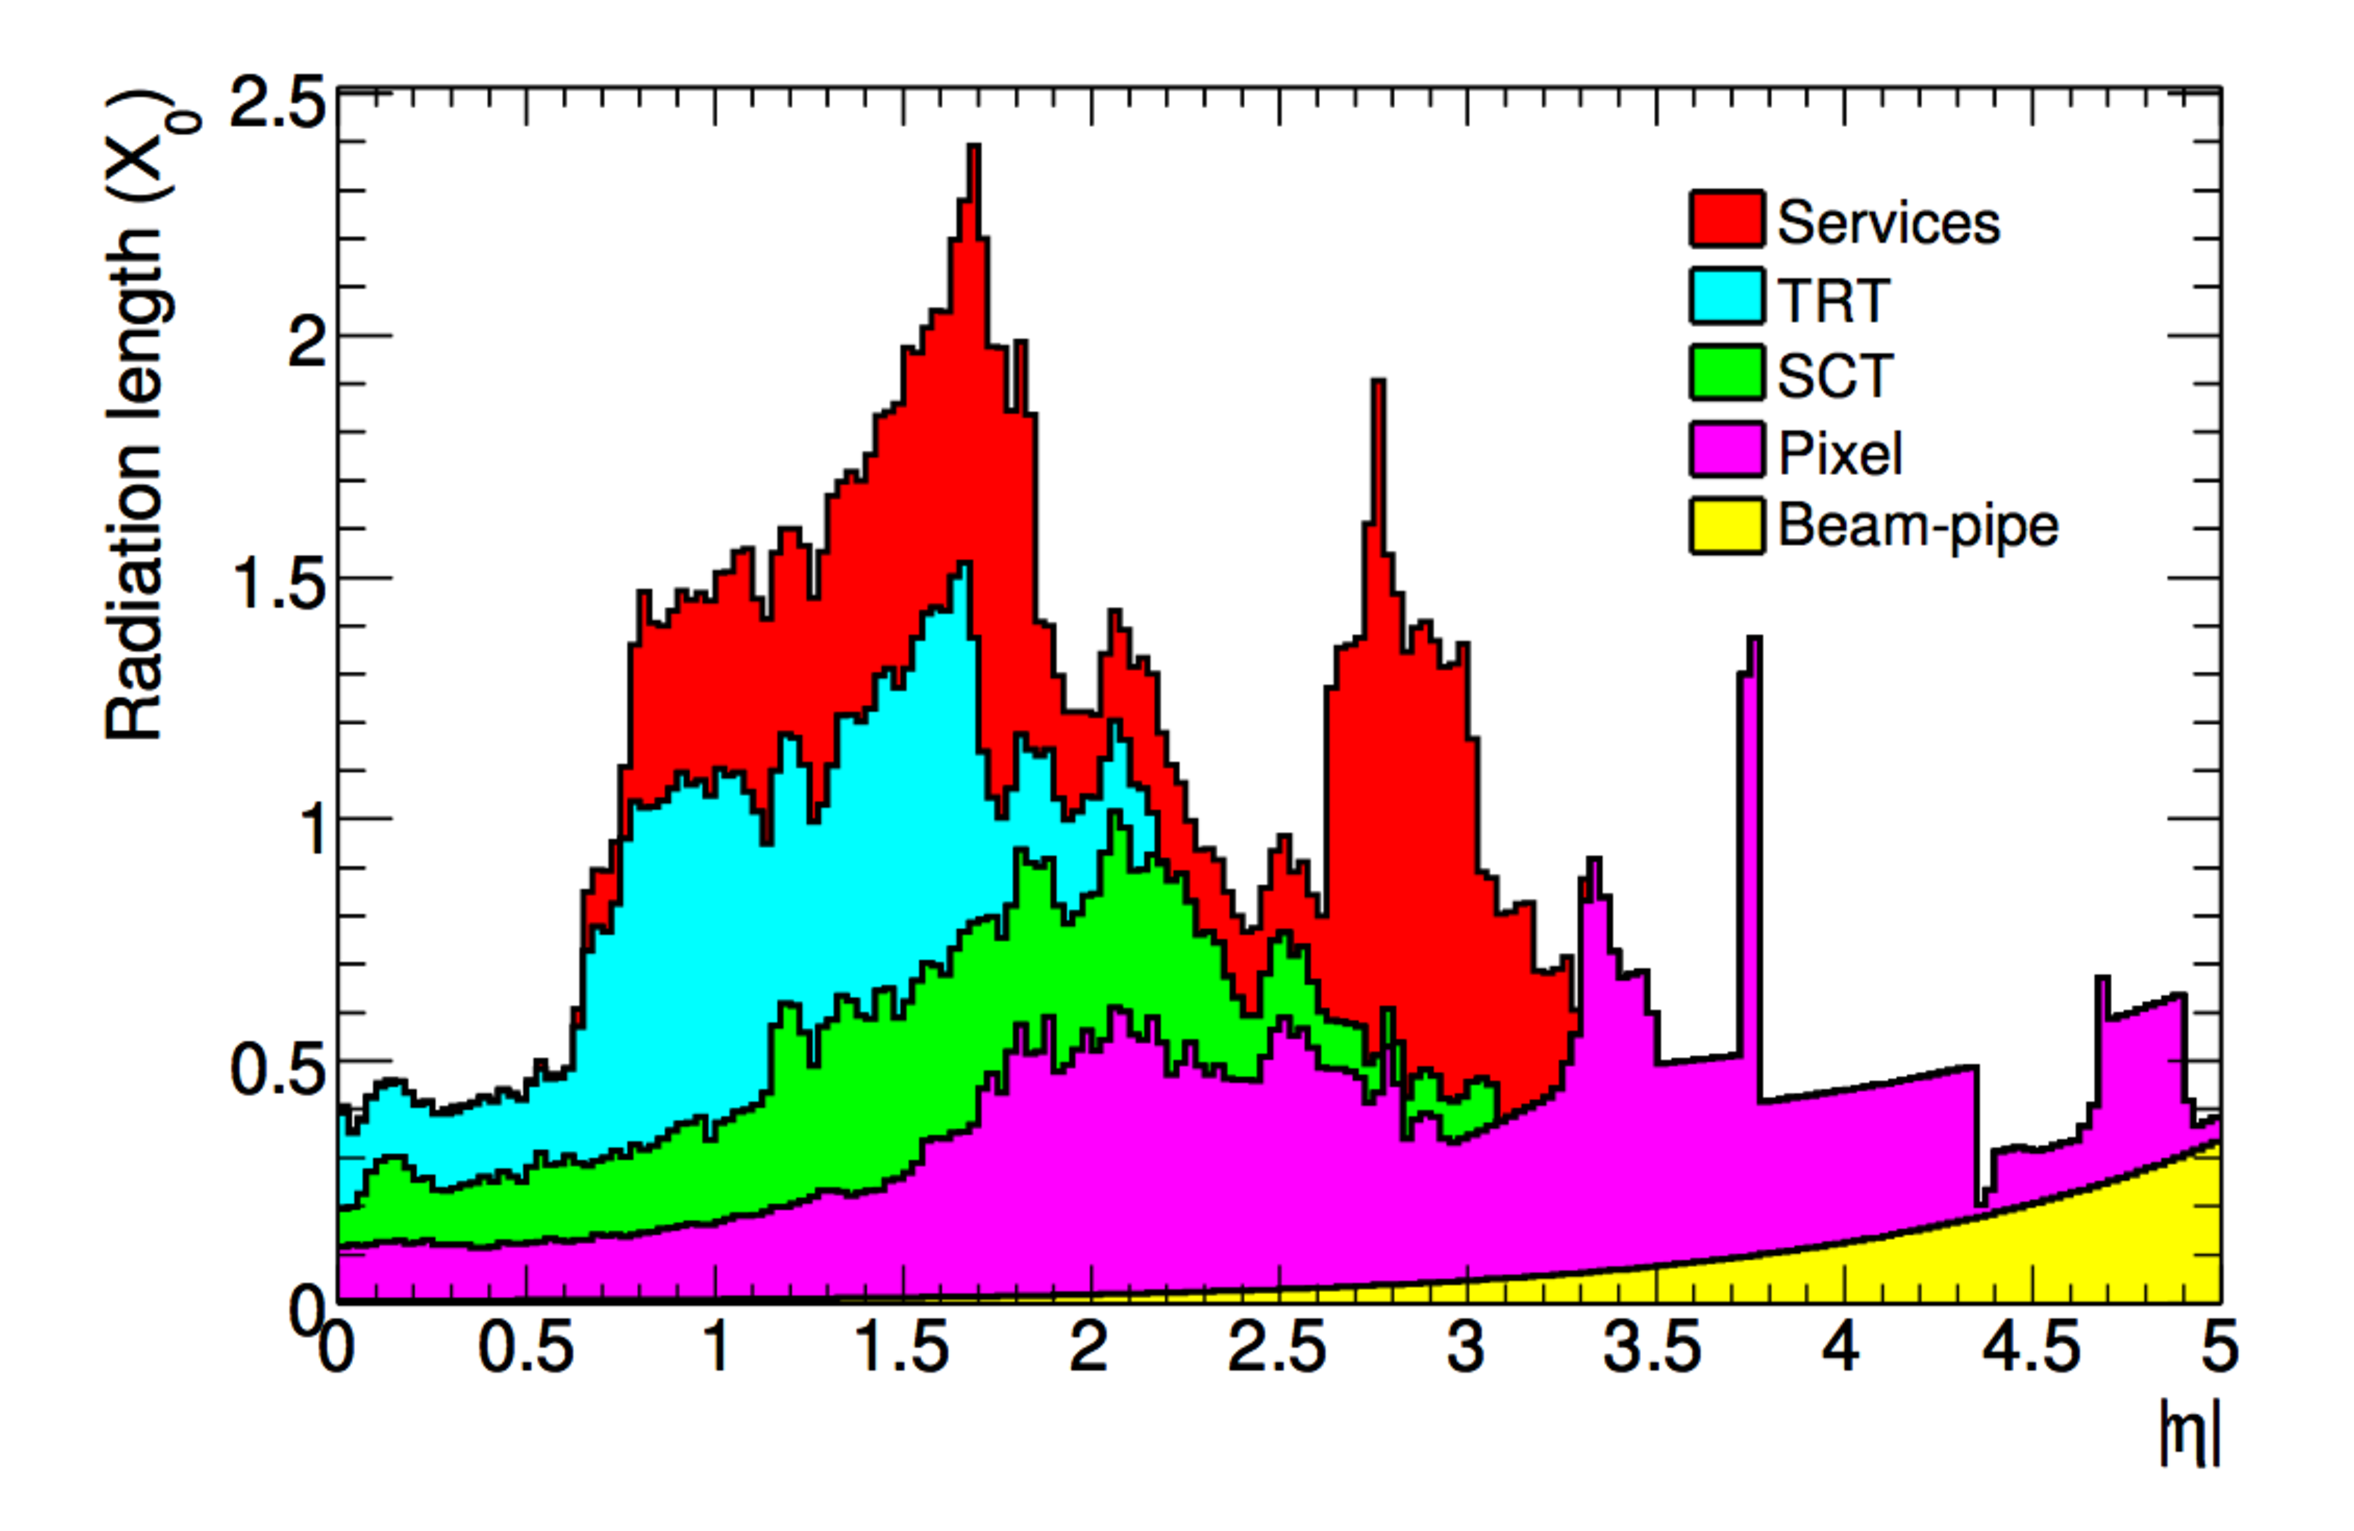
\includegraphics[width=0.48\textwidth]{figures/Detector/radLength_ID.pdf}}
    \subfigure[]{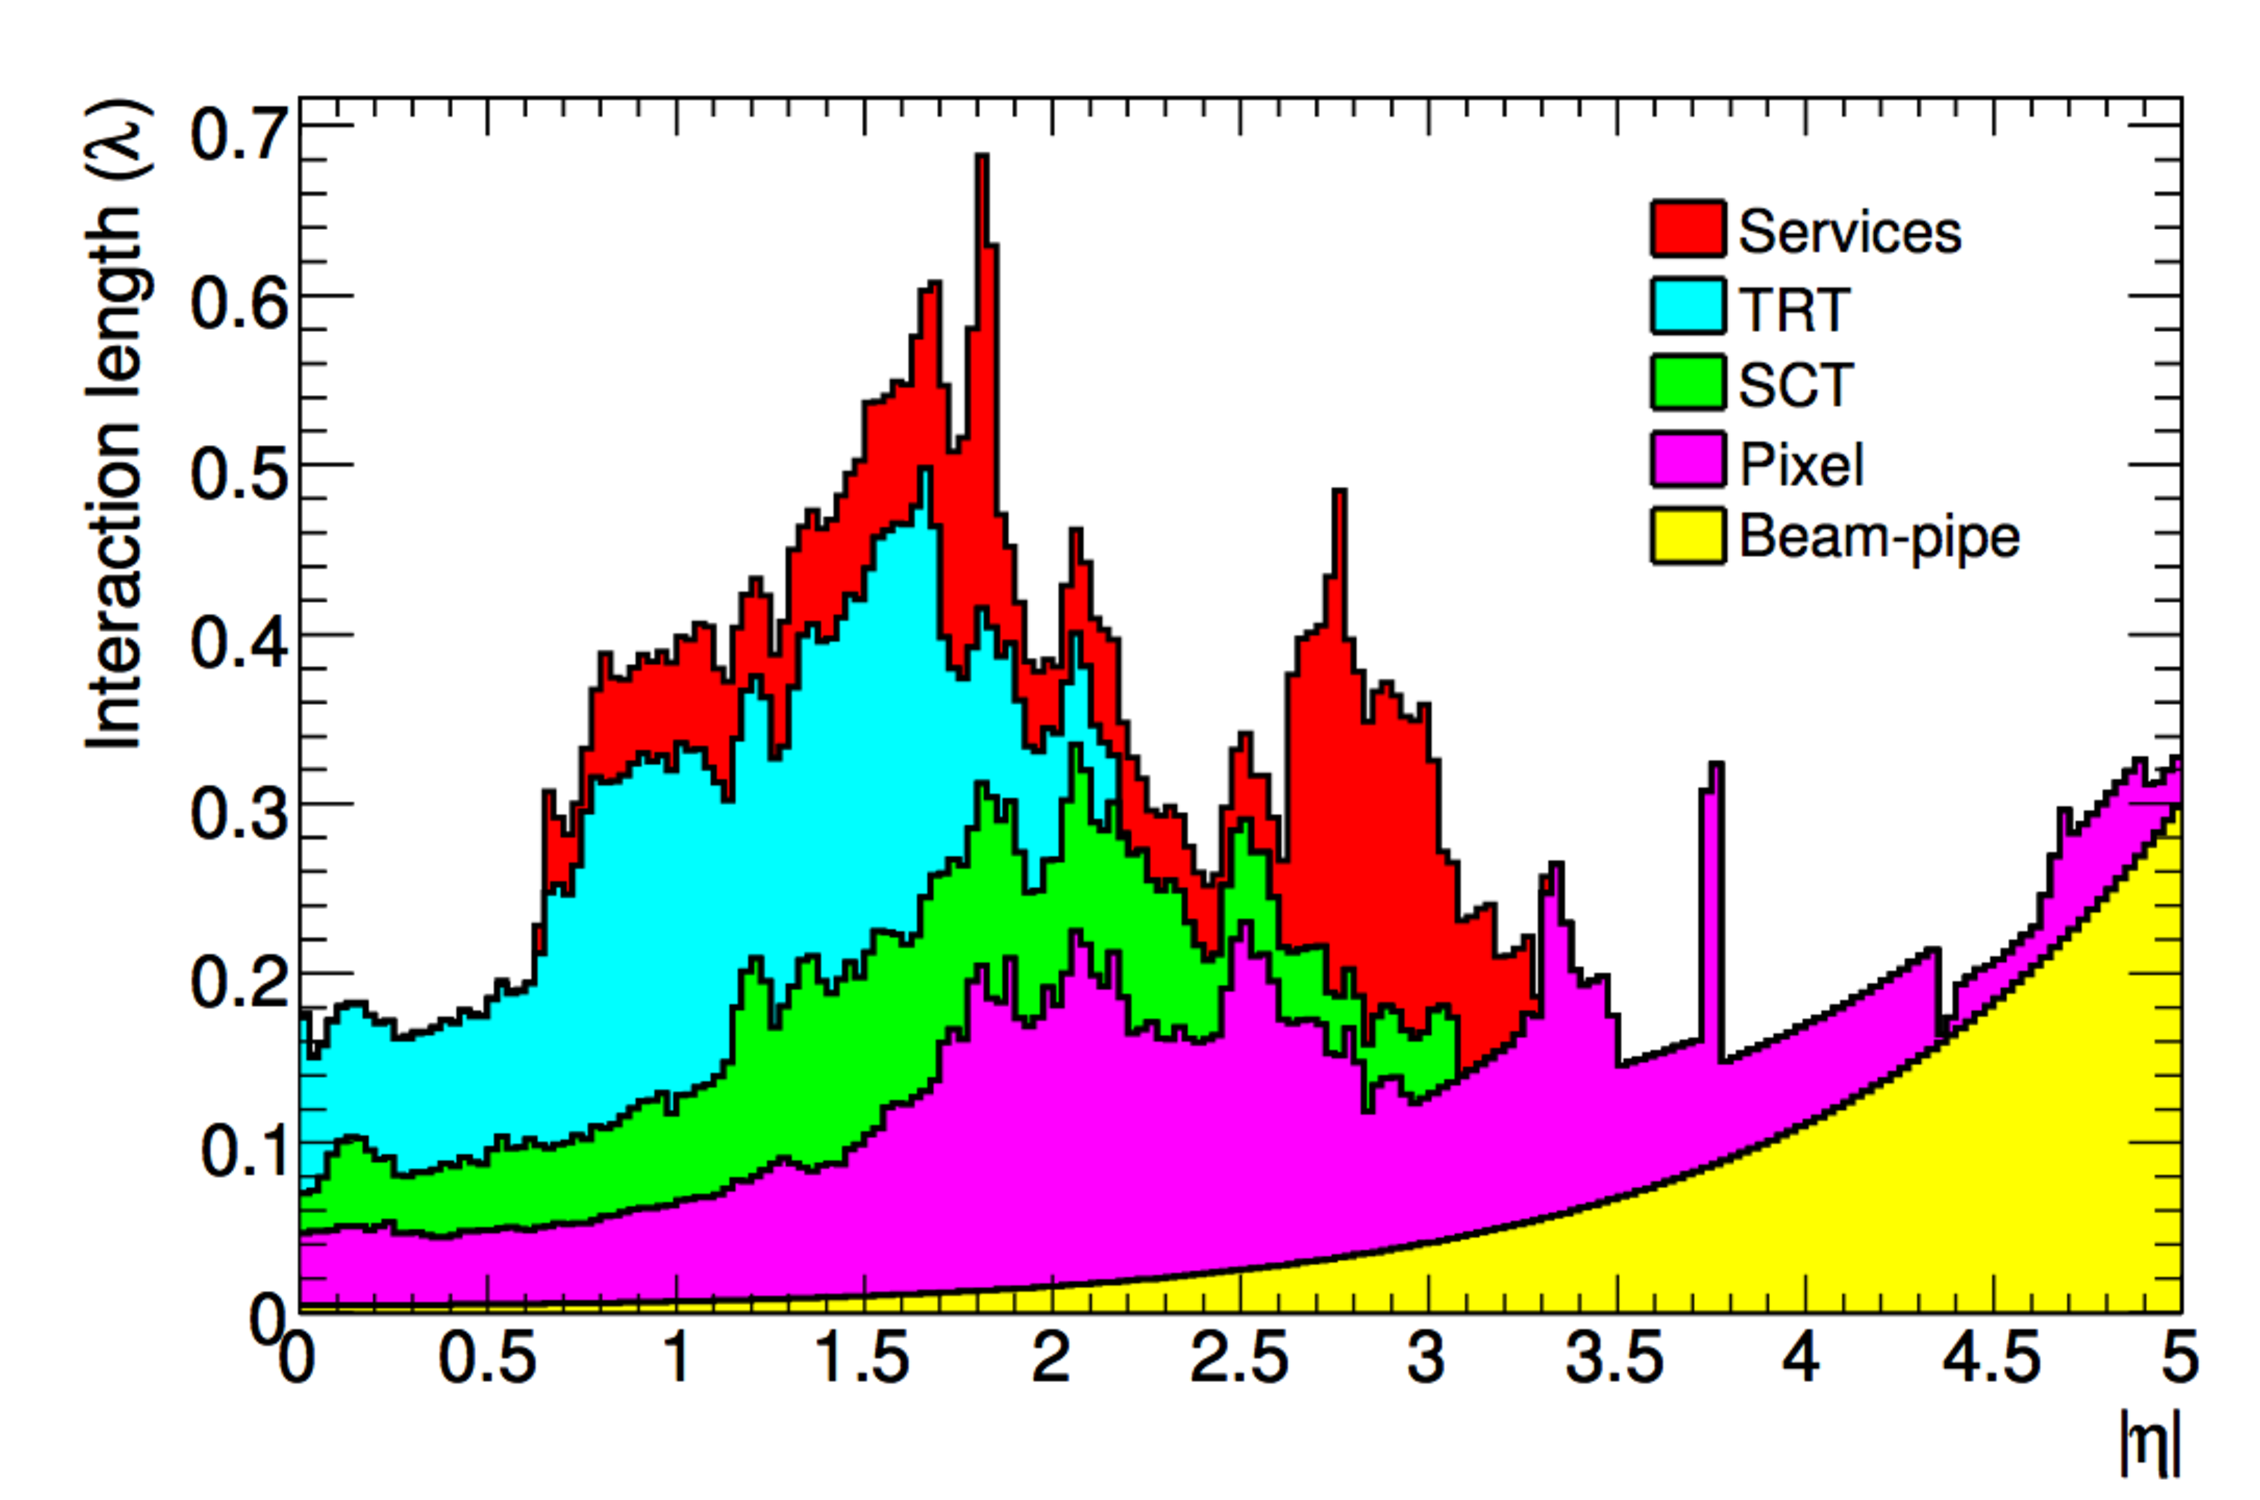
\includegraphics[width=0.48\textwidth]{figures/Detector/intLength_ID.pdf}}
    \caption{ Simulated material profile of whole ID in unit of (a) electro-magnetic radiation length and (b) nucleus interaction length \cite{ATLAS_exp}.
      Peak $|\eta|\sim 1.5$ corresponds to the barrel-endcap transition area through which service cables travel.
      \label{fig::Detector::IDmaterial} }
\end{figure}
%%%%%%%%%%



%%%%%%%%%%%%%%%%%%%%%%%%%%%%%%%%%%
\paragraph{The silicon trackers: Pixel and SCT} 
The detection principle of silicon detector is based on the electron-hole pair creation induced by a traverse of a charged particle.
%Thanks to the narrow band gap ($1.7 \mathrm{eV}$). 
Those electron-hole pairs are inhaled by the bias voltage applied on the sensor, and transferred into an electric signal. 
Silicon is particularly advantageous in 
The choice of silicon is largely for its radiation hardness durable the enormously high radiation around the IP. 
On the other hand, the performance (e.g. noise level, gain) is relatively sensitive to temperature, therefor they are kept in low temperature ($-5 \sim 0\deg$) during the operation.  \\

The pixel detector is the unit of layers of pixelated silicon sensors located closest to the IP of all the detector component. 
%The two-dimensional segmentation of the sensors gives space points without any ambiguities. 
Oxygen enriched n-in-n silicon semiconductor is used for the sensors.
Four cylindrical layers are placed in the barrel at the radial distance of 31 mm - 122.5 mm with respect to the IP, 
and 3 disk layers cover each side of the endcap, providing an acceptance with $|\eta|<2.5$. 
The innermost layer in the barrel is referred as the ``insertable b-layer'' (IBL) installed during the long shutdown between Run1 and Run2, providing the highest precision and playing a prominent role in identifying the secondary vertex of late decaying particles ($\tau$, $b$-hadrons etc.). 
The pixels are in the 50 $\times$ 250 $\um$ granularity in the IBL, and 50 $\times$ 400 $\um$ in the other layers. 
The resolution is purely determined by the pixel size. A spacial resolution of $4\um$ and $115\um$ is achieved along the radial and beam z-direction respectively, 
by combining the hit information from the four layers. \\

The SCT is located outside of the pixel detector. The sensors are made by single-sided p-on-n silicon semiconductors with 150 V of bias voltage applied. %要確認
The strips of barrel SCT aligning along the z-axis with $80\um$ pitch, giving a precision position in the $r-\phi$ plane. 
A slight angle stereo (40 mrad) alternated by layers is add to the arrangement, providing decent $z$-position determination in addition. 
The intrinsic resolution is $17\um (580\um)$ in $r-\phi (z)$ direction respectively.
%Each sensor has 768 strips readout individually.
The strips in the endcap SCT are aligned in a mesh in terms of $x-y$, capable of 3D position determination together with the $z$-coordinate of the disks.

%The total area coverage of silicon amounts up to $61m^2$, with 6.2 million readout channels.
% track 200um離れてれば分離可能
% thickness 285um

%%%%%%%%%%%%%


%基本的な流れ
%-前後とのつながり
%-一番小さいunitと検出動作原理, 読み出し, operation volrageとtemp, 素材への要求とか
%-それらがどう配置されてるか, geometryの特徴, hitの数とか
%-performance


%%%%%%%%%%%%%%%%%%%%%%%%%%%%%%%%%%%%%%%%%
%The pixel detector [1-9] is designed to provide a very high-granularity, high-precision set of measurements as close to the interaction point as possible. The system provides three precision measurements over the full acceptance, and mostly determines the impact parameter resolution and the ability of the Inner Detector to find short-lived particles such as B hadrons and τ lep- tons. The two-dimensional segmentation of the sensors gives space points without any of the ambiguities associated with crossed strip geometries, but requires the use of advanced electron- ic techniques and interconnections for the readout. The readout chips are of large area, with in- dividual circuits for each pixel element, including buffering to store the data while awaiting the level-1 trigger decision. Each chip must be bump-bonded to the detector substrate in order to achieve the required density of connections. In addition, the chips must be radiation hardened to withstand over 300 kGy of ionising radiation and over 5×1014 neutrons per cm2 over ten years of operation. The system contains a total of 140 million detector elements, each 50 μm in the Rφ direction and 300 μm in z, which are invaluable for the task of pattern recognition in the crowded environment of the LHC.
%The system consists of three barrels at average radii of ~4 cm, 10 cm, and 13 cm, and five disks on each side, between radii of 11 and 20 cm, which complete the angular coverage. The system is designed to be highly modular, containing approximately 1 500 barrel modules and 700 disk modules, and uses only one type of support structure in the barrel and two types in the disks.
%The pixel modules are designed to be identical in the barrel and the disks. Each module is 62.4 mm long and 21.4 mm wide, with 61 440 pixel elements read out by 16 chips, each serving an array of 24 by 160 pixels. The output signals are routed on the sensor surface to a hybrid on top of the chips, and from there to a separate clock-and-control integrated circuit. The modules are overlapped on the support structure in order to give hermetic coverage. The thickness of each layer is expected to be about 1.7% of a radiation length at normal incidence.
%
%%%%%%%%%%%%%%%%%%%%%%%%%%%%%%%%%%



%%%
%Each module consists of four . On each side of the module, two detectors are wire-bonded together to form 12.8 cm long strips. Two such detector pairs are then glued together back-to-back at a 40 mrad angle, separated by a heat transport plate, and the electronics is mounted above the detectors on a hybrid. The readout chain consists of a front-end amplifier and discriminator, followed by a binary pipeline which stores the hits above threshold until the level-1 trigger decision. The end-cap modules are very similar in construction but use tapered strips, with one set aligned radially. To obtain optimal η-coverage across all end-cap wheels, end-cap modules consist of strips of either ~12 cm length (at the outer radii) or 6-7 cm length (at the innermost radi- us).
%%%
%endcap diskは3種類 (inner/midle/outer)のdimension
%pn type  bias voltage


%%%%%%%%%%%%%%%%%%%%%%%%%%%%%%%%%%
\paragraph{Trasition radiation tracker}
% gas mixture
% TRTの原理もうちょい
% radiation at the boundary between two di-electric material s
TRT is a gaseous detector designed for tracking particles as well as identifying the species using the characteristic transition radiation.
The detector is filled with 4mm-diameter straw tubes in which xenon-based active gas is confined.
Ionized secondary electrons are collected by the $30\um$-diameter gold-plated tungsten-Rhenium anode wire in the center of each straws.
73 layers of aligned straw tubes are arranged in the barrel, and 160 layers in the endcap sectors. 
The tube length is 144 cm (37 cm) in the barrel (endcap) region. 
The barrel tubes are arranged in parallel along the beam pipe, with 7 mm of interval between layers.
The intrinsic position resolution per straw is about $130\mu m$.
A traverse of charged particle fires 36 straws on average, 

Transition material is inserted between the straws.
$19\um$-diameter polypropylene fibers are used in barrel, and $15\um$-thick polypropylene radiator foils isolated by a polypropylene net are set for the endcaps.
Transition radiation can address unique sensitivity in particle identification, particularly to  $e/\pi$ separation, 
since the intensity is sensitive to incident particle's velocity (proportional to $\gamma=E/m$) rather than the energy or momentum. 
Given that the signal of transition radiation typically yield more amplitude, in the TRT two differennt thresholds are set; 
the lower threshold to collect the signal of normal ionization and the high threshold for transition radiation. 
The high threshold is carefully designed so that only electrons can trigger in typical range of energy ($0.5\gev - 150 \gev$) while pions are inert to it. \\

Fig. \ref{fig::Detector::TRTPerf} shows the $\gamma$-dependence of high threshold rate, demonstrating good separation of particles with electron-like momentum and pion-like momentum.

%%%%%%%%%%%%%%
\fig[170]{Detector/TRTPerf.pdf}
{TRT high threshold rate as function of Lorentz factor ($\gamma=E/m$) of incident particles \cite{TRTPub}.
The $\gamma$ scale of typical pions and electrons are shown aside. Left/right plot corresponds to barrel/endcaps.}
{fig::Detector::TRTPerf}


%%%%%%%%%%%%%%%%%%%%%%%%%%%%%%%%%%
\paragraph{Combined Tracking Performance}
The combined tracking performance has been validated via measurement of the cosmic muons \cite{ATLAScosmicPerf}. 
The resolution for a single muon track is obtained as function of muon transverse momentum: 
% Typically, three pixel lay- ers and eight strip layers (four space points) are crossed by each track. A large number of track- ing points (typically 36 per track) is provided by the straw tube tracker (TRT) [1-8],
%The combination of two complental technologies provides very robust pattern recognition and high precision in
\begin{align}
\frac{\sigma_{\pt}}{\pt} = 1.6\% \oplus \frac{0.053\%}{\gev}\times \pt.  \label{eq::Detector::perf_ID}
\end{align}
%ATLAS_ID_performance_cosmic



%%%%%%%%%%%%%%%%%%%%%%%%%%%%%%%%%%%%%%%%%%%%%%%%%%%%%%%%%
\subsubsection{Calorimetery}
ATLAS includes two calorimeter systems composed of the electromagnetic calorimeter (EM calorimeter) and the hadronic calorimeter (HC), located outside the ID. 
The whole view is given by Fig. \ref{fig::Detector::calo}.
%The idea is ... to absorb the incident particles and  inside and calculate the energy deposit . intenseな物質とのhard interactionでcascade状シャワー作って
EM calorimeter, the inner part of the calorimetry, is aimed to measure energy of photons and electrons by causing them to EM shower. 
This is done by the Liquid-Argon sampling calorimeter (LAr), alternately sandwiching the lead absorber layers and the sensor layer filled with liquid-argon.
Most of the hadrons do not create EM showers and penetrate the EM calorimeter without major energy loss, which are then captured by the HC is placed the downstream. The HC exploits two detection technologies: the barrel HC, covering pseudo-rapidity range of $|\eta|<1.7$, is referred to the ``Tile calorimeter'' consisting of the sensor layers with scintillator tiles and steel absorbers; The endcap HC ($1.5<|\eta|<3.2$) employ the technology of LAr calorimeter similar to the EM calorimeter, however in a different geometry and coarser cell granularity. In addition to the EM calorimeter and HC, the forward calorimeter located in the very forward region ($3.2<|\eta|<4.9$) serve a supplemental function capturing the diffracted particles from jets. The detector technology used and the spatial segmentation are summarized in Tab. \ref{fig::Detector::caloSpec}.
Thanks to the fast response of the readout, calorimeter also provide the function of trigger, based on the fast processing of particle identification and the energy measurement using the information of individual showers, as detailed in Sec. \ref{sed::Detector::TDAQ}

\clearpage
\fig[140]{Detector/caloSpec.pdf}
{Summary of geometries for calorimeters \cite{ATLAS_TDR}.}
{fig::Detector::caloSpec}
\clearpage


\fig[110]{Detector/ATLAS_calorimeter.jpg}
{Cut-away view of the ATLAS calorimetery \cite{ATLAS_exp}.}
{fig::Detector::calo}



%%%%%%%%%%%%%%%%%%%%%%%%%%%%%%%%%%
\paragraph{Electromagnetic calorimeter}
%構造
%
% Basicなrequirementとしては, 
% Desnse material is preferred for absorber in general 
%e-piのPIDの観点からEGはECAL内で終わってほしいし、hadronはHCALでなるべくシャワーをスタートさせてほしい。そういうわけでradiation lengthの差は大きければ大きいほどよい。
The basic unit of LAr calorimeter consists of a gap filled with liquid argon (1.1-2.2mm) generating the ionized electrons, a copper-kapton electrodes to collect the ionized charge, 
and a steel-claded lead absorber layer to develop the EM shower (1.13-1.53mm). Bias voltage of 2000V between the electrodes and the absorbers is applied, achieving the drift time of 450ns. The detector is maintained at a constant temperature of $88K$ by the cryostats surrounding the barrel EM calorimeter. \\
%The readout current is tranfered into pulse signal ... 読み出しの話

%%%%%%%%%%
\fig[100]{Detector/LAr_cell.pdf}
{Geometry of barrel LAr sampling layers. 
Position resolution is addressed by the innermost sampling layer by the highest $\eta-\phi$ granularity of $0.0031\times0.098$,
and the energy measurement is mainly provided by the second layer with the largest volume.
The third layer standing behind in the plot is the tail catcher collecting the information of shower profile.
    \cite{ATLAS_TDR}.}
{fig::Detector::LArcell}
%%%%%%%%%%

The geometry and cell segmentation varies between barrel and endcap depending on the required function.
Fig. \ref{fig::Detector::LArcell} (b) illustrate the segmentation in the barrel ECM. 3 sampling blocks are placed along shower with different $\eta-\phi$ segmentation.
The first sampling layer has the finest $\eta-\phi$ granularity ($0.0031\times0.098$), identifying the precise angular position of the incident particle. The second sampling addresses the largest volume ($16X_0$) layer contains the most of shower in which the energy is mainly measured. The third sampling layer is intended to measure the very tail of EM showers, providing the information about longitudinal shower profile together with the other layers. \\
The layer units are arranged in an accordion geometry, which is the characteristic to the barrel ECM, designed to be fully hermitic in terms of angular acceptance. \\
%endcap EM calorimeterの特徴
%Only the latter two sampling layers are 

In order to compensate for upstream energy loss, a presampling layer is additionally located in front of the EM calorimeter for both barrel and the endcaps.
%with the thickness of 11 mm (5 mm) for barrel (endcap).

The total thickness amounts to $>22X_0$ in the barrel and  $>24X_0$ in the endcap, which can fully accommodate the EM showers of photons or electrons in an energy of a few TeV.
The transition region between the barrel and endcaps ($1.37 < |\eta| <1.52$) is dedicated to detector services and is thus not fully instrumented.

%needed for EG reconstruction -> fine segmentation , METの計算
%ATLASは特にpi0->gamgam veto(?)とconverted photonのIDに力入れてるので特にangular resolution に優れたECALになってる。
%3D showers are reconstructed by units of topo clustering

%sampled -> measured bipolar pulse shape transfer?
%pileup contribution should be subtracted all the time->negative biasing

The designed resolution is given in Eq. \ref{eq::Detector::perf_calo} \cite{ATLAS_LAr_TDR}:
\begin{align}
\frac{\sigma_E}{E} = \frac{10\%}{\sqrt{E}} \oplus \frac{17\%}{E} \oplus 0.7\%.
\label{eq::Detector::perf_calo}
\end{align}

The energy resolution for the off-line objects can be further improved through the dedicated calibration exploiting the full detail of the shower and the information from the other detector. 
This high pointing resolution is the characteristic advantage of the ATLAS EM calorimeter, which vastly benefits the particle identification (photon, high energy tau etc.) as well as MET reconstruction.



%%%%%%%%%%%%%%%%%%%%%%%%%%%%%%%%%%
\paragraph{Hadronic Calorimeter}
The ATLAS hadronic calorimeter consists of the barrel Tile HC ($|\eta|<1.7$) and endcap LAr HC.
The Tile HC is the sampling calorimeter composed by a periodic units of plastic scintillators tiles and steel absorber.
Fig. \ref{fig::Detector::caloCell} (a) schematizes one module in the Tile HC. Generated scintillation photons are read out by the photo-multiplier tubes equipped at the ends of the module via wavelength shifting fibers. 

Barrel Tile HC is segmented into three sections, the central barrel section ($|\eta|<1.0$) and the two extended barrel sections ($1.0<|\eta|<1.7$), using different channel dimensions. There are three sampling layers along the shower development with the thickness of 1.5$\lambda$, 4.1$\lambda$ and 1.8$\lambda$ for barrel, and 1.5$\lambda$, 2.6$\lambda$ and 3.3$\lambda$ for extended barrel respectively. \\

The endcap HC is the sampling calorimeter with liquid-argon sensor layers and copper absorber. 
The choice of material is dominantly based on the durablity against the extremely high radiation flux in the forward region.


The intrinsic resolution of barrel Tile HC and endcap LAr HC for an individual hadron jet is given as Eq. \ref{eq::Detector::perf_calo} \cite{ATLAS_Tile_TDR}: \\
% simulated ? measured?
%The gap between the sections is 4cm, in which the service cables for ID travel through.
\begin{align}
& \frac{\sigma_E}{E} = \frac{50\%}{\sqrt{E}} \oplus 3\%, \,\,\,\,\,\,\,\,\,\,\,\,  \mbox{(Tile HC)} \\
& \frac{\sigma_E}{E} = \frac{100\%}{\sqrt{E}} \oplus 10\%,  \,\,\,\,\, \mbox{(Endcap LAr HC)}
\label{eq::Detector::perf_calo}
\end{align}


%%%%%%%%%%%%%%%%%%%%%%%%%%%%%%%%%%
\paragraph{Forward Calorimeter}
A set of LAr calorimeter layers are arranged in a very forward region close to the beam axis covering $3.1<|\eta|<4.9$, 
designed to capture the full content from jets or particles from hard scattering particles from extremely boosted center-of-mass. The location with respect to the adjacent calorimeter systems are illustrated as Fig. \ref{fig::Detector::caloCell} (b).
Forward calorimeter is made by three sampling layers in which both functions of EM calorimeter and hadronic calorimeter are integrated; The first layer is with copper absorber working as EM calorimeter, and the later two layers are with tungsten functioning as EM calorimeter. An overlap with endcap HC is deliberated to realize smooth transition.

%%%%%%%%%%
\begin{figure}[h]
  \centering
    \subfigure[]{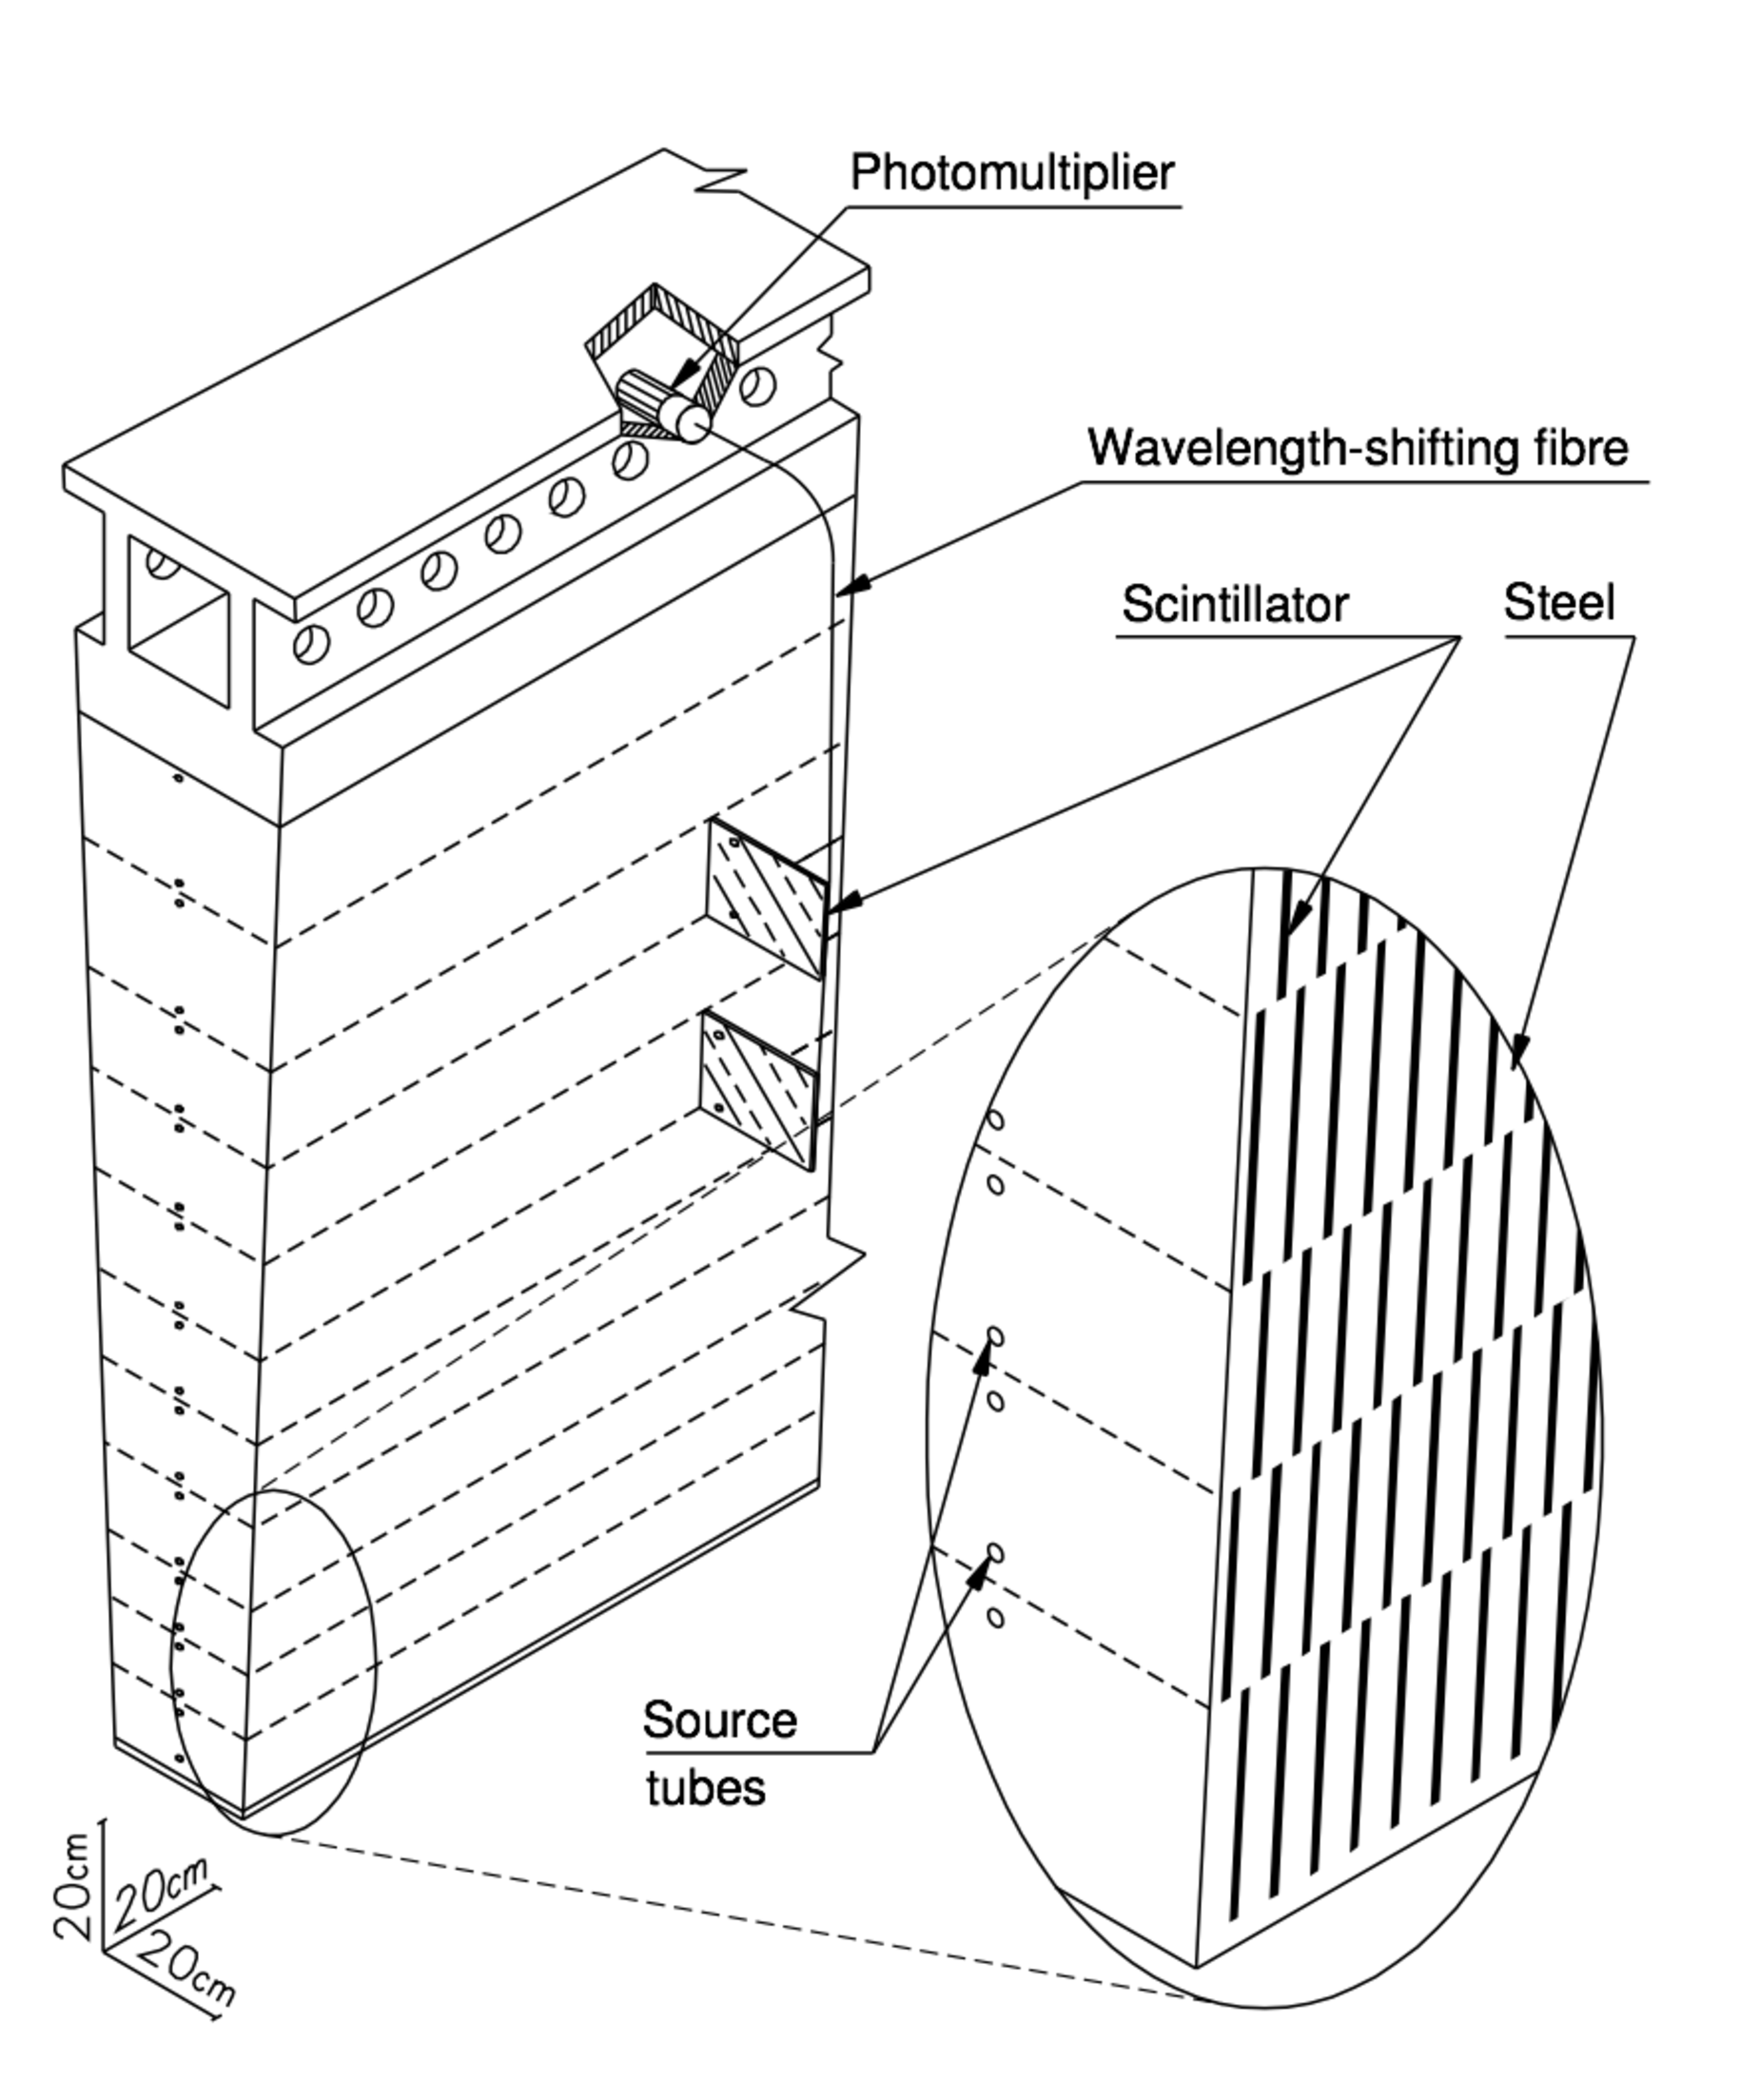
\includegraphics[width=0.415\textwidth]{figures/Detector/tile_cell.pdf}}
    \subfigure[]{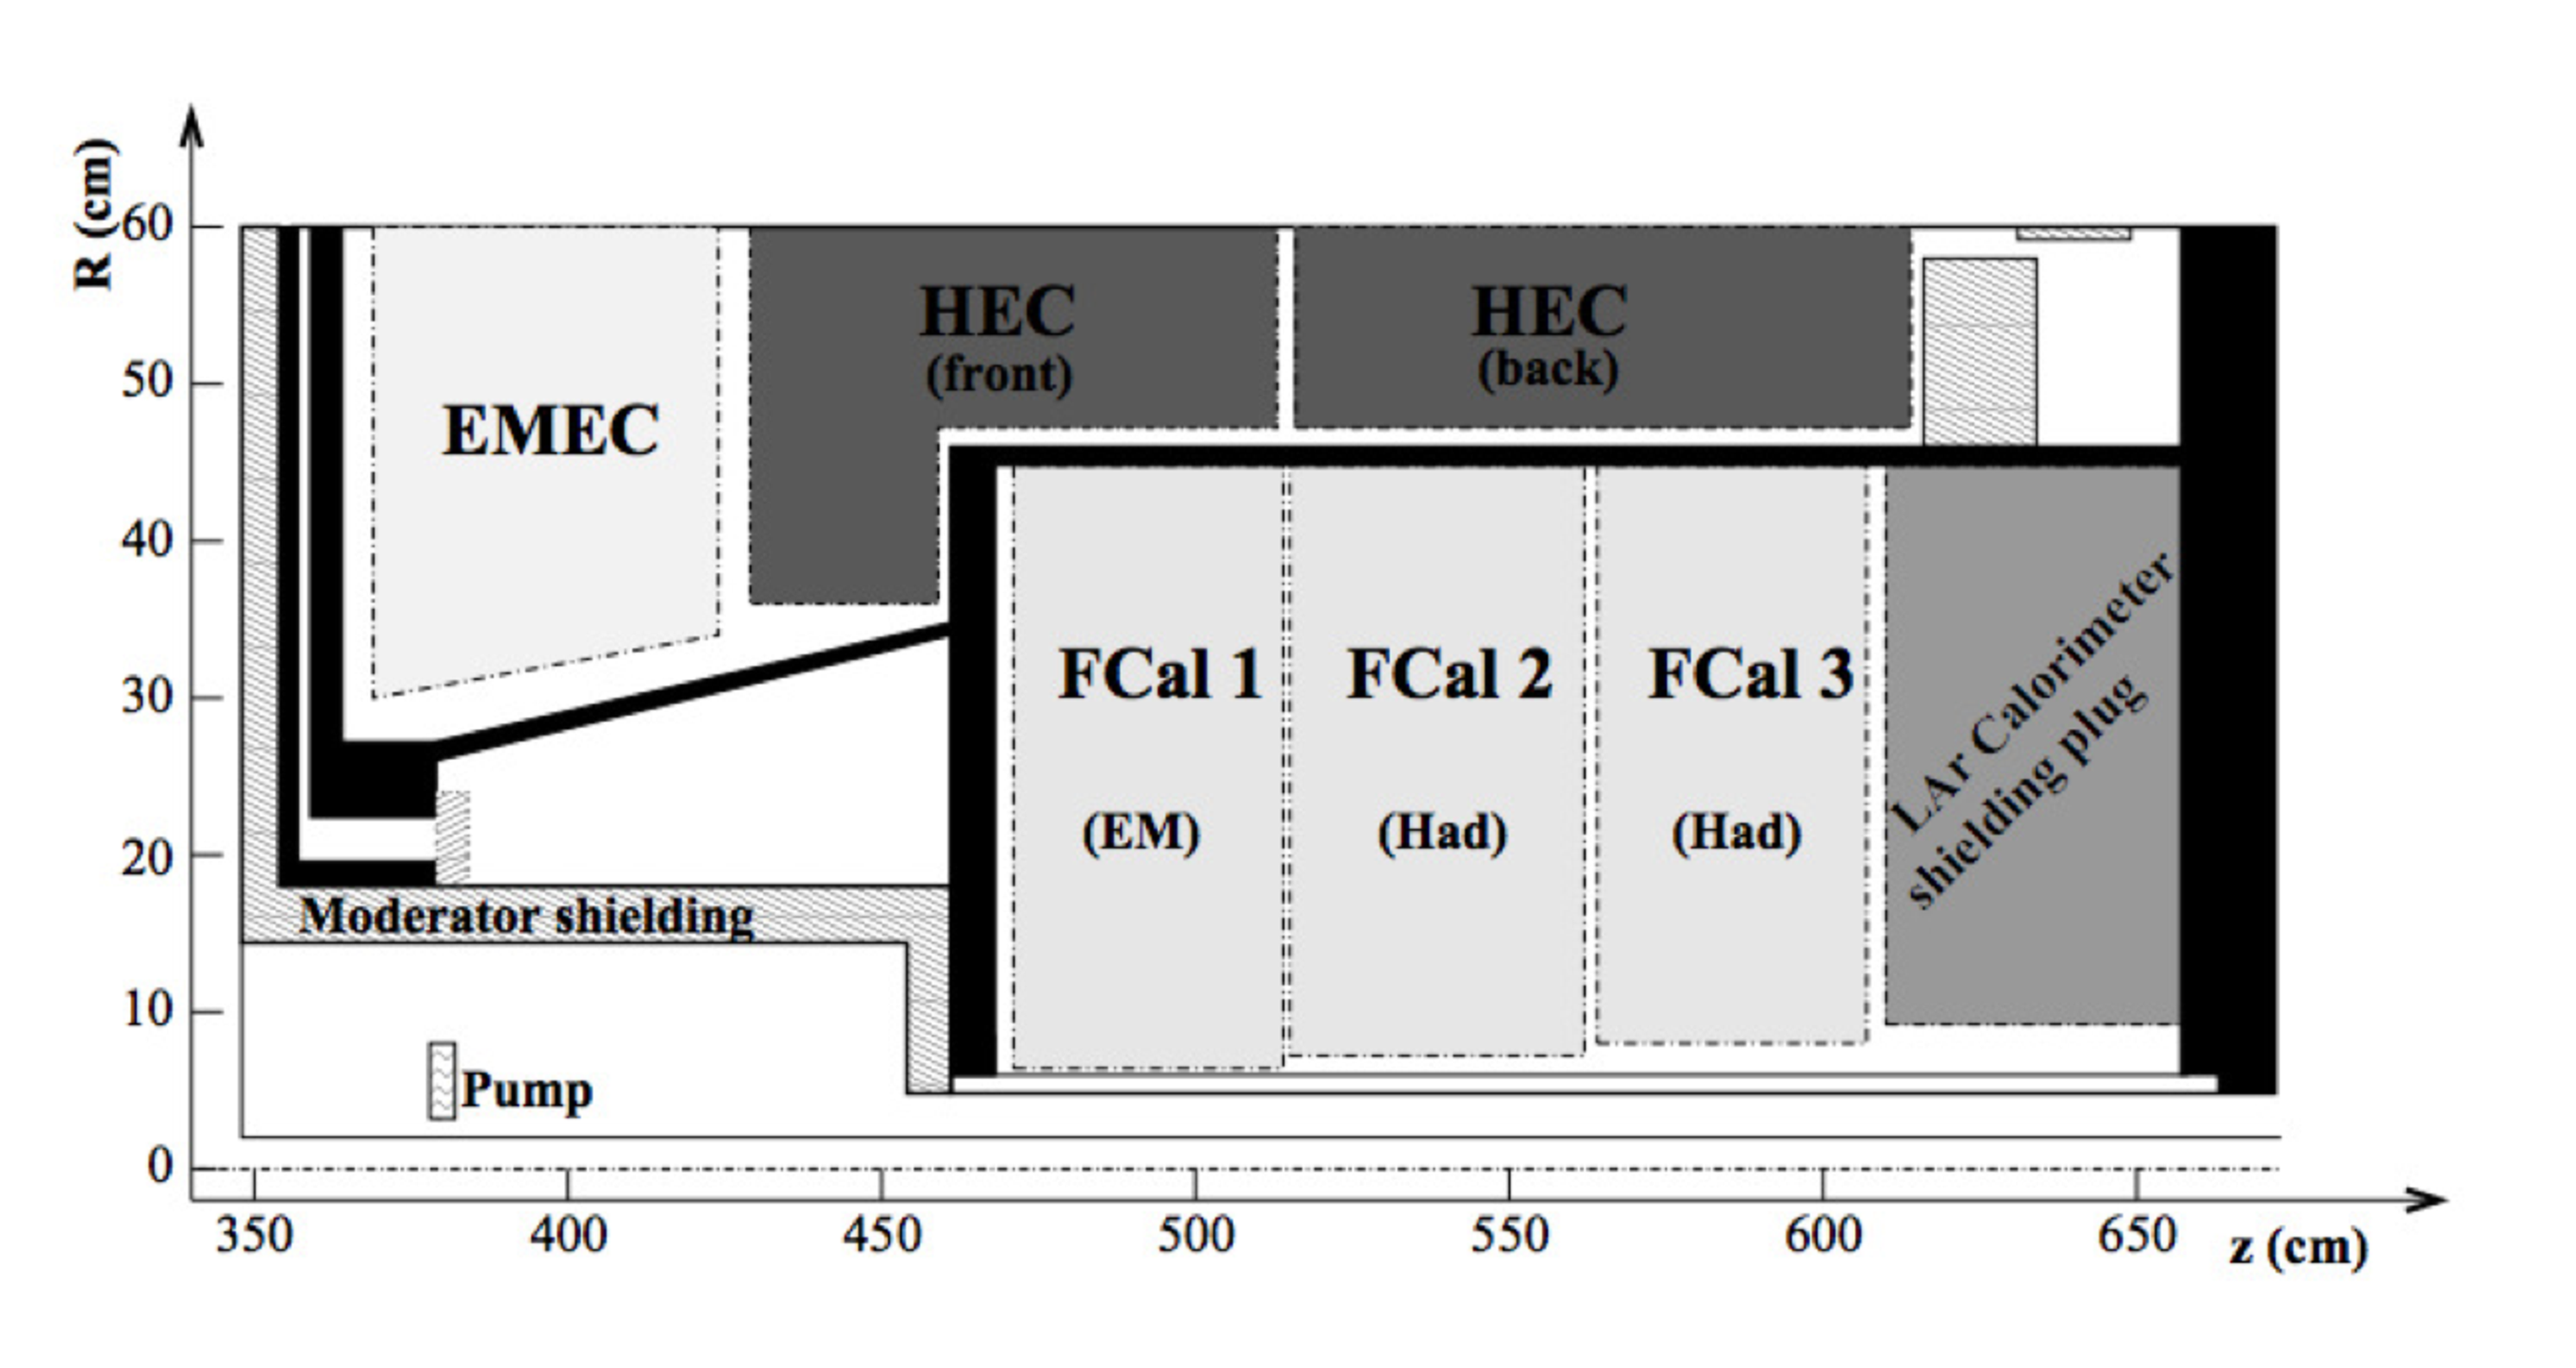
\includegraphics[width=0.575\textwidth]{figures/Detector/caloForward.pdf}}
    \caption{ (a) Illustration of a Tile HC module. (b)  Alignment of each detectors in an endcap; endcap LAr EM calorimeter (EMEC); endcap LAr Hadronic calorimeter (HEC); and the Forward calorimeter (FCal)   ) \cite{ATLAS_exp}.
      \label{fig::Detector::caloCell} }
\end{figure}
%%%%%%%%%%




%%%%%%%%%%%%%%%%%%%%%%%%%%%%%%%%%%%%%%%%%%%%%%%%%%%%%%%%%
\subsubsection{Muon Sspectrometer}
Muon spectrometers are located outermost in the ATLAS, consisting of four sub-detectors; Monitored Drift Tube (MDT); Cathode Strip Chamber (CSC); Resistive Plate Chamber (RPC); and the Thin-Gap Chamber (TGC). 
The former two are dedicated to precision measurement of muon tracks and the latter two are to triggering. 
The spectrometer covers the pseudo-rapidity range $ |\eta|< 2.7$ and allows identification of muons with momenta above 3 GeV and precise determination of $\pt$ up to about 1 TeV with $10\%$ momentum resolution.

The magnetic field for tracking is sourced by the three pieces of toroidal superconducting magnets; two end-cap toroids at the ends of the detector, and a barrel toroid embedded in the space inside the muon spectrometers. $3.9T$ and $4.1T$ B-field is provided in the barrel and endcap region respectively. The internal volume of toroidal coils are vacant (``air-core''), in order to reduce the material with which muons experience the multiple scattering, which is one of the limiting factors of the momentum measurement. The integrated B-filed profile at the position of MDT is shown in Fig. \ref{fig::Detector::BField_MDT}, while the global schematic of the magnet system is given in Fig. \ref{fig::Detector::magnet}.

\fig[110]{Detector/magnet_captioned.pdf}
{Schematic of the ATLAS magnet system with one central solenoid and 3 toroidals (barrel+2 endcaps). \cite{ATLAS_exp}.}
{fig::Detector::magnet}

%\fig[110]{Detector/magnet_photo.pdf}
%{Phono of ATLAS cross-seciotn.}
%{fig::Detector::magnet_photo}

\fig[110]{Detector/Bfield_MDT.pdf}
{ Simulated magnetic field integral provided by a single troid octant, from the innermost MDT layer to the outermost. \cite{ATLAS_exp}.}
{fig::Detector::BField_MDT}




%%%%
%momentum measurement from 3GeV to 1TeV (?), with 10% resolution at 1TeV
% |eta|<1.7 for barrel and 1.6<|eta1<2.7 for endcap
%toroidal, 8 coil per toroid
%∫B_T d_T: 1.5Tm-5.5Tm for barrel, 1Tm - 7.5Tm for endcap
%%%%

\paragraph{MDT}
MDT is a gaseous drift chamber filled with the basic detection elements of 30 mm-diameter aluminum tubes that are covered by a $400\um$ thickness wall. 
Drifting electrons are absorbed in the center of a tube by a $50\um$-diameter tungsten-Rhenium wire with a bias voltage of 3080V is applied, and read out by a low-impedance current sensitive preamplifier.
The gas mixture is tuned at Ar : $\mathrm{CO_2} ()$ = $93\%:7\%$, maintaining the maximum drift time of 700ns. The single wire resolution is $\sim 80\um$.
%In order to boost the number of hits per particle passage, the tubes are assembled in a layer, and the layers are stacked along the path of parcitles flight, forming a muti-layer, as schematized in Fig. \ref{}. 
There are three layers of MDT chambers located both in barrel and endcap, covering pseudo-rapidity range of $|\eta|<2.0$.
The limitation in the $\eta$-coverage is determined by its maximum durable rate ($150 cm^{-1}s^{-1}$), instead CSC takes over the role in the further forward region.
%% performance


\paragraph{Cathode Strip Cahmber}
%%読み出し
The CSCs are multi-wire proportional chambers covering the forward region ($|\eta|>2.0$) in the endcaps, providing 2D position of incident particles.
It is operated with a gas mixture of Ar $(80\%)$ and CO2 ($20\%$) and with a bias voltage of 1900V.
The cells are symmetric in terms of the pitch of readout cathodes and the anode-cathode spacing, which is equally set to 2.54 mm.
As the spatial resolution of the CSCs is sensitive to the inclination of tracks and the Lorentz angle, To minimize degradations of the resolution due to these effects, they will be the chamber is fixed at tilted posture so that tracks originating from the IP become orthogonal to the chamber surface.
%% performance


\paragraph{Resistiv Plate Chamber}
The RPCs are digital gaseous detectors specialized in fast timing response for triggering.
They are mechanically mounted on the surface in the barrel MDT, covering the pseudo-rapidity range of $|\eta|>1.05$.
The elementary detection unit is a gas gap filled with non-flammable gas mixture (94.7$\%$ $\mathrm{C_2 H_2 F_4}$, 5$\%$ $\mathrm{Iso-C_4 H_10}$, 0.3$\%$ $\mathrm{SF_6}$). An uniform high electric field ($\sim$ 4900 V/mm) is applied so that the ionized electrons amplitude by themselves by the avalanches. Signal is read out by a metal strip attached on both ends of the gaps, arranged with a pitch of 30 mm - 39.5 mm.
The typical spatial and timing resolution achieves 1 cm and 2 ns respectively.

%2 plates for measuring eta, phi position


\paragraph{Thin-Gap Chamber}
The TGCs are a special type of multi-wire proportional chambers characterized by the notably small distance between the anode wires and the read out cathode strips (1.4mm).
Together with the highly quenching gas mixture with $\mathrm{CO_{2}}$ ($55\%$) and n-pentan ($45\%$), a quick drain of secondary electrons is achieve with the timing response of 5 ns. TGCs also contribute to the momentum determination by supplementing the measurement in $\phi$ by MDT.
%A high voltage of 2900V is applied during the operation. 
Three modules are placed per endcap, covering $1.05<|\eta|<2.7$ by the innermost one and $1.05<|\eta|<2.4$ by the two behind. Trigger is generated using tracks in $1.05<|\eta|<2.4$, while all tracks are utilized for momentum measurement.


\fig[110]{Detector/ATLAS_muonDetector.pdf}
{Global view of the ATLAS muon spectrometers \cite{ATLAS_exp}.}
{fig::Detector::muon}


\fig[110]{Detector/muon_xsec2.pdf}
{Cross-section of the ATLAS Muon spectrometer \cite{ATLAScosmicPerf}.}
{fig::Detector::muon_xesc2}



%%%%%%%%%%%%%%%%%%%%%%%%%%%%%%%%%%%%%%%%%%%%%%%%%%%%%%%%
\subsubsection{Luminosity Detectors}
Luminosity determination is particular important since it provides the reference in normalizing simulated dataset and enables the sensible comparison to data. 
The instantaneous luminosity is calculated the formula below:
\begin{align}
\mathcal{L} = \frac{\mu n_b f_b}{\sigma},
\end{align}
where $n_b$ is the number of colliding crossinges and the $f_b$ the frequency of the beam circulation.
$\sigma$ is total fiducial cross-section of $pp$ interaction including both elastic and inelastic scattering, and $\mu$ is the average number of such interaction per crossing crossing. While $\sigma$ is provided by a dedicated calibration measuring the lateral beam profile using overlapping two beams referred as the van der meer scan \cite{VdMScan}, $\mu$ is obtained directly by exploiting the rate information from luminosity detectors located in the very forward region nearby the beam pipe. Dedicated calibration and luminosity determination algorithm studied in \cite{LumiMeasurement}.

%Three luminosity detectors contribute to the luminosity measurement:
Two luminosity detectors mainly contribute to the luminosity measurement:
\begin{description}
%\item[BCM] (Beam Conditions Monitor) \\

\item[LUCID] (LUminosity measurements using Cherenkov Integrating Detector) \\
LUCID are located at the both ends of the ATLAS detector at a distance of 17m from the IP, covering the pseudo-rapidity range of $5.6<|\eta|<6.0$.
The LUCID detector consists of 16 aluminum tubes filled with $\mathrm{C}_4 \mathrm{F}_{10}$ gas, 
and designed to count the Cherenkov photons kicked out by charged particles flying along the beam axis which are mainly generated by proton-proton inelastic scattering in the IP.
The measurement is translated into luminosity, which is used for online monitoring of the instantaneous luminosity as well as the beam condition. 
%collcted by the photomultiplier set in the back-end

%array of 20 Cerenkov tubes (?) 
%pp非弾性散乱から来る破片のcharged particleの数を数える


\item[ALFA] (Absolute Luminosity For ATLAS) \\
ALFA is located beyond the ATLAS envelope at $z=\pm 240$ m, sandwiching the beam pipe from top and bottom.
The detectors are composed of 8 scintillating fibers, designed to mainly measure the elastic scattering component of the $pp$ interaction.

%小角のpp弾性散乱で飛んで来たpを測る. optical theoremでtotal cross-sectionわかるので、
\end{description}



%%%%%%%%%%%%%%%%%%%%%%%%%%%%%%%%%%%%%%%%%%%%%%%%%%%%%%%%%
\subsubsection{Trigger and Data Acquisition System}
While ATLAS enjoys incredibly high collision rate of about 100 MHz (40 MHz beam crossing crossing together with pile-up),
these data cannot entirely read out due to the limitation from data transmission as well as the computation resource.
Luckily or unluckily, most of them are junk QCD reactions resulting in cheap low $\pt$ jets, 
the rate can be drastically suppressed by requiring hard jets, leptons or $\met$ in the events.

A highly sophisticated data acquisition system have been developed for ATLAS, referred as ATLAS Trigger and Data Acquisition System (TDAQ) \cite{trigger2015}, handling the trigger and readout. The schematic of the readout stream is shown in Fig. \ref{fig::Detector::triggerFlow}.
It consists of a two-staged trigger pipeline served by the hardwere-based Level-1 Trigger (L1) and the software-based High-Level Trigger (HLT).
The idea is to reject the major trivial QCD events in L1, based on a fast particle reconstruction with a coarse resolution, and perform further filtering in HLT based on using more sophisticated reconstruction and energy measurent, enjoying the timing latency that L1 earns. The benchmark of rate suppression is 100 kHz at the end of L1 and down to 1 kHz after the HLT on average. \\
The L1 consists of two independent sub-trigger systems: L1Calo, identifies the EM or hadronic clusters in calorimeter and reconstruct primitive jets, electrons, photons and taus (L1 objects) with calibrated energy in EM scale.; L1Muon, identifies and measure the tracks in the muon spectrometer, designed to accept events with muons. 
The object reconstruction is based on the coarsely segmented blocks of combined detector channel called ``trigger tower'' with $\eta\times\phi$ granularity of $0.1 \times 0.1$. 
%RoIの話も?
$\met$ is also calculated at the L1 stage by the vectorial sum of the calorimeter deposits, referred as L1XE. Trigger accept is issued by the Central Trigger Processors (CTP) when the L1 objects meet certain criteria in terms of $\pt$ thresold and number of objects.  \\

In HLT, an offline-like algorithm is employed to refine the energy of L1 objects, or recover the mis-identified objects (typically low $\pt$ muons) by scanning over whole detector. This is performed by a set of custom farmwares with a processing time of 0.2 s on an average. The event that is triggered by the HLT is subsequently sent to event storage infrastructures outside the ATLAS. 
Fig. \ref{fig::Detector::trigger_ratePhys} illustrates the acception rate of HLT in 2016 operation. \\

The performance of triggers relevant to the analysis is dedicatedly overviewed in Sec. \ref{sec::Samples::trigger}.

%Relevant trigger chains to the thesis is shown as Tab. \ref{}.
%The $\met$ trigger is used as the main trigger.
%The single-lepton triggers supplement the 

% HLTはofflineにかなり近いparticle reconstruction/identification/calibrationを使う
%
\fig[110]{Detector/triggerFlow.pdf}
{The logic of ATLAS trigger system \cite{trigger2015}. Trigger detectors have separated readout line for trigger, sending input information for trigger decision to CTP. 
CTP reconstruct L1 objects and issue a global accept signal relieving the buffered data, once the trigger criteria are satisfied. 
The $(\eta,\phi)$ position of identified trigger object is sent to downstream HLT, in which off-line like software based trigger runs to filter events further.
L1 topological trigger (L1 Toplo) and Fast Tracker (FTK) have been in commissioning since 2015. 
%L1Topo is designed to offer triggers exploiting the event topology information (e.g. azimuthal angle difference between two particles) using the combined output from L1Calo and L1Muon. FTK is the hardware-based fast tracking module working in the L1 time designed to feeding the reconstructed tracks HLT.
}
{fig::Detector::triggerFlow}

\fig[110]{Detector/trigger2016_physicsRate.png}
{Rate of HLT stream for physics analysis during the 2016 data-taking \cite{trigPubResult}. Horizontal axis is in unit of lumi-clock, the smallest unit of data-taking in the same configuration.}
{fig::Detector::trigger_ratePhys}



%%%%%%%%%%%%%%%%%%%%%%%%%%%%%%%%%%%%%%%
\subsection{Recorded Data by ATLAS}
The $pp$ collision data analyzed in the thesis were collected by ATLAS during 2015 and 2016 at a centre-of-mass energy of 13 TeV. 
The evolution of the peak luminosity and  corresponding average pileup increase are shown in Fig. \ref{fig::Detector::DAQ}.

Data-quality requirements are applied based on each lumi-block, the smallest unit of data-taking defined as the period in the run configuration which varies conditions of beam and detector. 
Rejected data is typically at the period with more than a certain of fraction of modules in the sub-detectors being disabled or in a wrong operation voltage.
Integrated luminosity delivered by LHC and recorded in ATLAS during the 2016 operation is shown in Fig. \ref{fig::Detector::dataInt}. After the quality requirement the luminosity of data used for analysis is to $32.9\ifb$, to which $3.2\ifb$ from 2015 data taking is added, amounting to $36.1\ifb$ with the measurement error of $\pm3.2\%$. \\

\fig[110]{Detector/intLumi2016.png}
{Evolution of integrated luminosity delivered by LHC (green) and recorded in ATLAS (yellow) in 2016 oepration \cite{DAQ2016}.}
{fig::Detector::dataInt}

